\documentclass{report}

\usepackage[T1]{fontenc}

\usepackage{url}
\usepackage{minitoc} \setcounter{minitocdepth}{1}
\usepackage{verbatim}
\usepackage{graphicx}

\title{{\Huge \bfseries PyZUI}\\Manual}
\author{David Roberts}

\begin{document}
  \maketitle
  \dominitoc
  \faketableofcontents

  \begin{abstract}
  PyZUI is an implementation of a Zooming User Interface (ZUI) for Python.
  Media is laid out upon an infinite virtual desktop, with the user able to pan
  and zoom through the collection.

  PyZUI is compatible with the following media formats:
  \begin{itemize}
    \item All images recognised by ImageMagick\footnote{
            \url{http://imagemagick.org/script/formats.php}
          }
    \item PDF documents
    \item Remote webpages
    \item SVG (vector graphics)
  \end{itemize}

  Raster images of arbitrary size can be viewed due to the use of image
  tiling\footnote{
    \url{http://star.pst.qub.ac.uk/idl/Image_Tiling.html}
  }. The largest image tested so far is the 233 megapixel Blue Marble Next
  Generation 2km/pixel satellite image\footnote{
    \url{http://earthobservatory.nasa.gov/Features/BlueMarble/images_bmng/2km/
         world.topo.bathy.200407.3x21600x10800.jpg}
  }.

  PyZUI also allows viewing of remote media from the following online services:
  \begin{itemize}
    \item OpenStreetMap\footnote{
            \url{http://openstreetmap.org/}
          } (world-wide street directory)
    \item The WMS Global Mosaic\footnote{
            \url{http://onearth.jpl.nasa.gov/};
            1.3TB, max. resolution 15m/pixel
          } (NASA satellite imagery)
  \end{itemize}

  Examples of similar projects include Seadragon/DeepZoom\footnote{
    \url{http://livelabs.com/seadragon/};
    Presentation: \url{http://ted.com/index.php/talks/
                       blaise_aguera_y_arcas_demos_photosynth.html}
  }, OpenZoom\footnote{
    \url{http://openzoom.org/};
    Demonstration: \url{http://tandem.gasi.ch}
  }, Zoomorama\footnote{
    \url{http://zoomorama.com/}
  }, and Eagle Mode\footnote{
    \url{http://eaglemode.sf.net/}
  }. More basic ZUIs can also be found in software such as Compiz and Spaces
  (included in Mac OS X), as well as devices such as the Nintendo Wii and Apple
  iPhone. A more complete listing of other projects can also be found at
  Wikipedia\footnote{
    \url{http://en.wikipedia.org/wiki/ZUI}
  }.
  \end{abstract}

  \chapter{User Interface}
  Upon startup of PyZUI, the user is presented with the \emph{home scene}, as
  shown in Figure \ref{fig:home_scene}.

  \begin{figure}[h!]
  \begin{center}
    
\includegraphics[width=10cm]{../images/home_scene.png}
    \caption{Home Scene} \label{fig:home_scene}
  \end{center}
  \end{figure}

  The menus provide the following actions:
  \begin{description}
    \item[File]
    \begin{itemize}
      \item \textbf{New Scene (Ctrl+N)} Create a blank scene
      \item \textbf{Open Scene (Ctrl+O)} Open a saved scene
      \item \textbf{Open Home Scene (Ctrl+Home)}
            Return to the \emph{home scene}
      \item \textbf{Save Scene (Ctrl+S)} Save the current scene
      \item \textbf{Save Screenshot (Ctrl+H)}
            Export the current viewport to an image
      \item \textbf{Open Local Media (Ctrl+L)} Open media from a local file
      \item \textbf{Open Media by URI (Ctrl+U)}
            Open media identified by a URI \\
            The following URI formats are recognised:
            \begin{itemize}
              \item any valid URL e.g. \url{http://google.com/}
              \item \url{dynamic:mandel}: the Mandelbrot set
              \item \url{dynamic:osm}: OpenStreetMap
              \item \url{dynamic:gm}: the WMS Global Mosaic
              \item \url{dynamic:fern}: the PyZUI logo (aka Barnsley's fern)
              \item \url{string:rrggbb:foobar}:
                    a string, where \url{rrggbb} is a string of three two-digit
                    hexadecimal numbers representing the colour of the text,
                    and \url{foobar} is the text to be displayed \\
                    e.g. \url{string:00ff00:hello} will display ``hello'' in
                    green
            \end{itemize}
      \item \textbf{Open Media Directory (Ctrl+D)}
            Open the media contained in a directory, and arrange it into a grid
            (see Figure \ref{fig:grid})
            \begin{figure}[h!]
            \begin{center}
              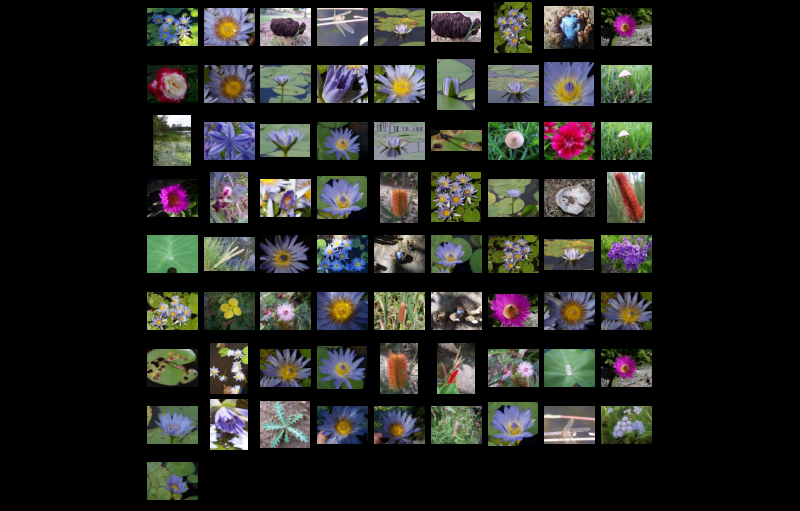
\includegraphics[width=10cm]{../images/grid.png}
              \caption{Media directory} \label{fig:grid}
            \end{center}
            \end{figure}
      \item \textbf{Quit (Ctrl+Q)} Exit the application
    \end{itemize}
    \item[View]
    \begin{itemize}
      \item \textbf{Set Framerate}
            Set the rendering framerate to the selected frequency
      \item \textbf{Fullscreen (Ctrl+F)} Toggle fullscreen mode
    \end{itemize}
    \item[Help]
    \begin{itemize}
      \item \textbf{About} Show PyZUI copyright information
      \item \textbf{About Qt} Show Qt about dialog
    \end{itemize}
  \end{description}

  \pagebreak

  The following mouse/keyboard actions are also available:
  \begin{description}
    \item[Left-click] Select the foremost media under the cursor
    \begin{itemize}
      \item if there is no media under the cursor then the currently selected
            media will be deselected
      \item if the Shift key is currently being held then no change will be
            made to the current selection
    \end{itemize}
    \item[Click`n'drag] Select and move the foremost media under the cursor
    \begin{itemize}
      \item if there is no media under the cursor then the currently selected
            media will be deselected and the entire scene will be moved
      \item if the Shift key is currently being held then no change will be
            made to the current selection and the entire scene will be moved
    \end{itemize}
    \item[Esc] Deselect the currently selected media
    \item[PgUp/PgDn or Scrollwheel] Zoom the currently selected media
    \begin{itemize}
      \item if there is no currently selected media, or if the Shift key is
            currently being held, then the entire scene will be zoomed
      \item if the Alt key is currently being held, then the zoom amount will
            reduced allowing for finer control
      \item Note: the point under the cursor will maintain its position on the
            screen
    \end{itemize}
    \item[Arrow keys] Move the currently selected media in the specified
                      direction
    \begin{itemize}
      \item if there is no currently selected media, or if the Shift key is
            currently being held, then the entire scene will be moved
      \item if the Alt key is currently being held, then the move amount will
            reduced allowing for finer control
    \end{itemize}
    \item[Space bar] Move the point under the cursor to the centre of the
                     screen
    \begin{itemize}
      \item holding the Space bar allows panning by moving the cursor around
            the centre of the viewport
    \end{itemize}
    \item[Del] Delete the currently selected media
  \end{description}

  \chapter{Class Design}
  \minitoc
  \input{apidoc.tex}

  \chapter{Dependencies}
  PyZUI depends on the following packages:
  \begin{itemize}
    \item PyQt4
    \item Python Imaging Library (PIL)
    \item ImageMagick
    \item pdftoppm
    \item jrMandel
  \end{itemize}

  For further information see the \texttt{INSTALL.txt} file, which is
  replicated below:
  {\footnotesize\verbatiminput{../../INSTALL.txt}}
  
  \chapter{Efficiency}
  To judge the efficiency of the application, a small script
  (\texttt{test/benchmark.py}) was written and run on eight images\footnote{
    The first three images are from an average digital camera. The fourth and
    eighth are satellite imagery from NASA:
    \url{http://earthobservatory.nasa.gov/Features/BlueMarble/images_bmng/8km/
         world.topo.bathy.200407.3x5400x2700.jpg};
    \url{http://earthobservatory.nasa.gov/Features/BlueMarble/images_bmng/2km/
         world.topo.bathy.200407.3x21600x10800.jpg} \\
    The remaining images are from \emph{Life In Megapixels}:
    \url{http://lifeinmegapixels.com/location.php?location=gorne};
    \url{http://lifeinmegapixels.com/location.php?location=mscnt};
    \url{http://lifeinmegapixels.com/location.php?location=kingsn}
  } of various sizes on a machine with a 1.73GHz CPU and 512MB RAM. The results
  of this are summarised in the following table (for full results see
  \texttt{test/benchmark.log}):

  \begin{center}
  \begin{tabular}{l|c|c|c|c}
    \textbf{Image} & \textbf{1} & \textbf{2} & \textbf{3} & \textbf{4} \\
    Area (megapixels) & 3.54 & 3.98 & 4.98 & 15 \\
    Width (px) & 2304 & 2304 & 1932 & 5400 \\
    Height (px) & 1536 & 1728 & 2580 & 2700 \\
    Conversion time & 0.66s & 0.70s & 0.88s & 3.02s \\
    Tiling time & 1.81s & 1.91s & 2.56s & 7.95s \\
    Tiling memory use (MB) & 4.81 & 4.49 & 3.80 & 8.04 \\
    Cold zooming mean FPS & 20 & 21 & 21 & 21 \\
    Warm zooming mean FPS & 26 & 27 & 27 & 28 \\
    \hline
    \textbf{Image} & \textbf{5} & \textbf{6} & \textbf{7} & \textbf{8} \\
    Area (megapixels) & 35 & 75 & 160 & 233 \\
    Width (px) & 11756 & 22194 & 20634 & 21600 \\
    Height (px) & 3009 & 3367 & 7751 & 10800 \\
    Conversion time & 1m52s & 13m23s & 2m33s & 3m9s \\
    Tiling time & 27s & 1m8s & 1m31s & 2m11s \\
    Tiling memory use (MB) & 5.79 & 19 & 31 & 33 \\
    Cold zooming mean FPS & 13 & 10 & 19 & 18 \\
    Warm zooming mean FPS & 30 & 41 & 29 & 27 \\
  \end{tabular}
  \end{center}

  \section{Conversion}
  It can be seen that the conversion time for the first three average sized
  images is negligible, and not overly significant for the 15MP image. For the
  other four images, the conversion time is much more significant, especially
  in the case of image 6 which took 13m23s.

  This anomaly is likely because of the way in which ImageMagick caches pixel
  data\footnote{
    \url{http://imagemagick.org/script/architecture.php}
  } during the conversion. For smaller images, the pixel data is cached
  directly in RAM. However, once the image size passes a certain threshold,
  it is cached to disk instead. On the machine this was tested on, the
  ``automagically'' determined default threshold is 740MB.

  For the Q16 version of ImageMagick, each pixel in the image consumes 8 bytes
  in the pixel cache. Therefore, the first 5 images consumed 29MB, 32MB, 40MB,
  120MB and 280MB respectively, meaning that they could be stored entirely in
  RAM. The last 2 images consumed 1.3GB and 1.9GB respectively, meaning that
  they would be cached to disk instead. However, image 6 consumed 600MB ---
  below the threshold, but larger than the amount of physical memory available.
  Therefore, ImageMagick would have attempted to cache this image to the
  machine's virtual memory, but as it was larger than RAM a portion of it would
  have been required to be swapped to disk, causing the system to thrash, hence
  accounting for the substantial time taken.

  Also, although the 280MB consumed by image 5 could theoretically be stored
  entirely within in the 512MB of RAM, in practice a substantial amount of the
  available RAM would be occupied by other applications. Therefore the
  conversion of this image may have also caused minor thrashing. This is
  evident in the much longer conversion time when compared to the first 4
  images.

  If this situation were likely to be an issue, the user could alter the
  configuration of ImageMagick to lower the threshold to a reasonable value.
  PyZUI could also be altered to attempt to alter the threshold value itself,
  but this would not necessarily result in optimal values being set.

  It is likely that thrashing caused by the conversion of images 5 and 6 may
  have impacted on the rest of the benchmarking of those images. Therefore they
  will be counted as a anomalies and will not included in the calculations in
  the following sections.

  \section{Tiling}
  \subsection{Time}
  Inspecting the values given in the above table shows that tiling time is
  almost directly proportional to the area of the image --- performing a
  linear regression results in a coefficient of determination ($R^2$) of
  $\sim0.99994$. From this it can be tentatively assumed that the tiling
  process has a time complexity of $\Theta(n)$, where $n$ is the area of the
  image.

  Running \texttt{benchmark.py} on image 8 with profiling enabled (using the
  \texttt{cProfile} module), shows that 76\% of the tiling time was spent
  loading pixels from the file (\texttt{Tiler.\_\_load\_row\_from\_file}), and
  another 21\% of the tiling time was spent saving tiles to disk
  (\texttt{Tiler.\_\_savetile}) --- a total of 97\% of tiling time being spent
  on these IO operations. As both of these operations are proportional to the
  size of the image, this agrees with the time complexity assumed in the
  previous paragraph.

  \subsection{Space}
  Similarly, inspecting the values in the table shows that that tiling memory
  usage is almost directly proportional to the \emph{width} of the image
  ($R^2\approx0.9988$). From this it can be tentatively assumed that the tiling
  process has a space complexity of $\Theta(w)$, where $w$ is the width of the
  image.

  This agrees with the fact that only a single row is processed at a time, and
  since every row has a height of 256px, the memory consumed by each row is
  proportional to the width of the image.

  \section{Rendering}
  The difference between the efficiency of cold and warm rendering should
  be noted. In this context, cold rendering means the tile cache began empty,
  and warm rendering means most of the required tiles were already in the tile
  cache when rendering began. This difference in rendering framerate shows the
  increase in efficiency provided by the tile caching mechanism.

  Discounting the anomalies discussed previously, it can be seen that all
  images have approximately the same rendering framerate independent of image
  size. The larger images have a slightly reduced cold rendering framerate, but
  this is only because they required tiles to be loaded from disk for higher
  resolutions, whereas the other images simply resized existing tiles
  in-memory. This shows how tiling images allows arbitrarily large images to be
  rendered efficiently.

  \section{Possible Improvements}
  The \texttt{Tiler.\_\_load\_row\_from\_file} method is optimised for memory
  usage, by only loading a single line of pixels from the file at a time.
  However, as discussed previously, this method accounts for around 75\% of the
  total tiling time. Therefore, it may be beneficial for a compromise to be
  made between memory usage and time efficiency, possibly by loading larger
  chunks of pixel data at a time.

  Rendering efficiency could be improved by adding support for rendering with
  OpenGL. However, this would not replace the current rendering system since
  OpenGL is not currently supported by all video cards.

  SVGMediaObject is very slow at rendering complex SVG files. This could be
  improved by implementing an SVGTileProvider which renders tiles on demand and
  provides them to a TiledMediaObject. This would improve the responsiveness of
  the application as SVG rendering would be performed in the background, and
  tile caching would mean that the SVG file need not be rendered for every
  frame.

\end{document}
